%\begin{enumerate}[label=\thesection.\arabic*.,ref=\thesection.\theenumi]
%\numberwithin{equation}{enumi}
\item An aircraft roll control system can be represented by a block diagram shown in Fig. \ref{fig:es17btech11002_block} with G\brak{s} in feedback system, whose error  $K_v$ = 5. Determine K 
\begin{align}
G\brak{s} &= \frac{10K}{s\brak{s+1}\brak{s+5}}
\label{eq:es17btech11002_system}
\end{align}
%\item 
The block diagram is given by Fig.\ref{fig:es17btech11002_block}
\begin{figure}[!ht]
 \centering
     \resizebox{\columnwidth}{!}{
\tikzstyle{block} = [draw, fill=white!20, rectangle, 
    minimum height=3em, minimum width=4em]
\tikzstyle{sum} = [draw, fill=white!20, circle, node distance=1cm]
\tikzstyle{input} = [coordinate]
\tikzstyle{output} = [coordinate]
\tikzstyle{pinstyle} = [pin edge={to-,thin,black}]
\begin{tikzpicture}[auto, node distance=2cm,>=latex']
    % We start by placing the blocks
    \node [input, name=input] {};
    \node [sum, right of=input,node distance=2cm] (sum) {$\sum_{}^{}$};
    \node [block, right of=sum] (controller) {$C(s)$};
    \node [block, right of=controller,
            node distance=2.5cm] (system) {G(s)};
    % We draw an edge between the controller and system block to 
    % calculate the coordinate u. We need it to place the measurement block. 
    \draw [->] (controller) -- node[name=u] {} (system);
    \node [output, right of=system] (output) {};
    \coordinate [below of=u] (tmp);

    % Once the nodes are placed, connecting them is easy. 
    \draw [draw,->] (input) -- node  {$X(s) $} (sum);
    \draw [->] (sum) -- node {$ $} (controller);
    \draw [->] (system) -- node [name=y] {$Y(s) $}(output);
    \draw [->] (input) -- node{$ $} node[pos=0.93]{$+$} (sum);
    \draw [->] (y) |- (tmp) -| node[pos=0.99] {$-$} 
        node [near end] {$ $} (sum);
    
\end{tikzpicture}
}
    \caption{}
    \label{fig:es17btech11002_block}
\end{figure}
%\\

%\item \solution 
For unity feedback we have Velocity error constant $\brak{K_v}$
\begin{align}
K_v &= \lim_{s \to 0} s G\brak{s} 
\end{align}
\begin{align}
\lim_{s \to 0} \brak{\frac{10K}{\brak{s+1}\brak{s+5}} }& = 5 \\
\implies K = 2.5
\end{align}
It's Phase Margin  = 3.94\degree\\
and Gain Crossover Frequency = 2.03 rad/s
Refer Fig. \ref{fig:es17btech11002_1} for plot G\brak{s}.
\begin{lstlisting}
codes/es17btech11002_1_new.py
\end{lstlisting}
\begin{figure}[!h]
\centering
  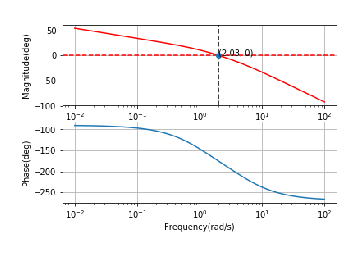
\includegraphics[width=\columnwidth]{./figs/es17btech11002_1_new.eps}
  \caption{}
  \label{fig:es17btech11002_1}
\end{figure}

%\item Design a Lag-Lead Compensator to yield a Phase margin\brak{PM} of 60\degree \\
%\solution 
Compensator required phase angle \brak{\phi_{m}} and  Phase Margin Frequency \brak{\omega_{pm}}, 
\begin{align}
    \phi_{m}= -\brak{180\degree+\theta}+PM+5 & =65\degree
    \\
    \omega_{pm}=1.25 rad/s.
\end{align}
Attenuation factor $\brak{\alpha\beta}$ is given by
\begin{align}
\alpha= 0.5
\\
\beta =  20
\end{align}
Lead and Lag Compensator Design Parameter is given in TABLE \ref{table:es17btech11002_1}
\begin{table}[!ht]
\centering
\input{./table/es17btech11002_1_new.tex}
\caption{Zeroes and Poles}
\label{table:es17btech11002_1}
\end{table}
And Compensator obtained has transfer function
\begin{align}
    G_{c}\brak{s}= \frac{\brak{s+0.279}\brak{s+0.125}}{\brak{s+5.590}\brak{s+0.00625}}
\end{align}

%\item Plot the graph after adding Lead-Lag compensator.
%\\
%\solution 
Refer Fig\ref{fig:es17btech11002_2} for plot $G\brak{s}G_{c}\brak{s}$.
\begin{lstlisting}
codes/es17btech11002_2_new.py
\end{lstlisting}
\begin{figure}[!h]
\centering
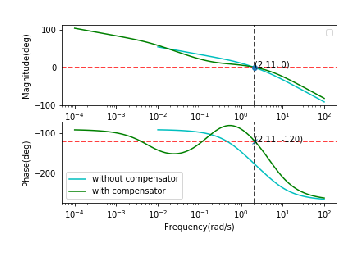
\includegraphics[width=\columnwidth]{./figs/es17btech11002_2_new.eps}
\caption{}
\label{fig:es17btech11002_2}
\end{figure}

\textbf{NOTE :} The idea of using a lead-lag network is to provide the attenuation of a phase-lag network and the lead-phase angle of a phase-lead
network. This points should be noted while designing a controller, and parameters to be changed accordingly to get exact results.
%\end{enumerate}     
